\part{Using Git on your own}

\section{Using Git on your own}

\begin{frame}
\frametitle{Using Git on your own}
\begin{itemize}
    \item Why would you want to use Git alone?
    \item You obtain benefits of version control, e.g.:
        \begin{itemize}
            \item Have a safety net and access to a time machine.
            \item Get a log of changes over time and why.
            \item In the future, you can return to previous work and
                understand what your thoughts and ideas were.
        \end{itemize}
    \item You can use Git on your own computer, hence:
        \begin{itemize}
            \item setup and management is quick and simple,
            \item there are no servers to administer,
            \item no cloud service is necessary.
        \end{itemize}
    \item There are even more benefits when working with others; we'll
        discuss this in more detail later in the course.
\end{itemize}
\end{frame}

\section{Example project: a kiwi café}

\subsection{Getting started}

\begin{frame}{Example project: kiwi café}
Let's discover how Git can be useful with the help of a concrete example.

    \textbf{Introducing:}
    \begin{quote}
        Kiwi Cakes and Coffee\\
        Great coffee, awesome cake.
    \end{quote}

    \textbf{Scenario:}\\
    You're the proud owner of a new café with a focus on cake recipes found
    in New Zealand.
\end{frame}

\begin{frame}{Initial thoughts}
Where to start?
    \begin{itemize}
        \item The café is a big project.
        \item You'll want to collect the cake recipes
            somewhere sensible on your computer.  You and your staff
            can then find them easily.
        \item You'll probably want to store other information about your
            café close to the cake recipes.
        \item Thus, it makes sense to create a directory for the café and a
            subdirectory for the cake recipes.
    \end{itemize}
\end{frame}

\begin{frame}[fragile]{Project structure}
Create the project directories by running the following commands:
\begin{shellcode}
    mkdir kiwi-cakes-and-coffee
    cd kiwi-cakes-and-coffee
    mkdir recipes
\end{shellcode}

You now have this directory structure:
\begin{minted}{console}
    kiwi-cakes-and-coffee/
    └── recipes
\end{minted}

    Great!  A well-organised directory layout is a good first step.  Now we
    need to add some recipes.
\end{frame}

\subsection{A first recipe}

\begin{frame}[fragile]{A first recipe}
    Let's start with a classic that works anywhere: chocolate cake.

    \begin{itemize}
        \item Enter the \code{recipes} directory
        \begin{shellcode}
            cd recipes
        \end{shellcode}
        \item Open a new file in your text editor called \code{chocolate-cake.md}.
    \end{itemize}
\end{frame}

\begin{frame}[fragile]{A first recipe}
    Fill the file with this text
    (\href{https://raw.githubusercontent.com/paultcochrane/git_course/refs/heads/master/git/examples/edmonds-chocolate-cake.md}{\beamerbutton{link}}):
    \inputminted[fontsize=\tiny]{markdown}{examples/edmonds-chocolate-cake.md}
    {\footnotesize \emph{Edmonds Cookery Book}, 51st De Luxe Edition, 2003.}
\end{frame}

\begin{frame}{Why use Git?}
    \begin{itemize}
        \item We're likely to change recipes in the future.
        \item We'll also want to add and remove recipes.
        \item We'll need a system to store the files and manage the changes: Git.
        \item Thus, we need to create a Git repository in
            \code{kiwi-cakes-and-coffee} directory.
    \end{itemize}
\end{frame}

\subsection{Side note: concerning repositories}

\begin{frame}{What is a repository?}
    But first, what \emph{is} this repository thing?

    \begin{description}
        \item[repository] /ripózzitəri, -tri/, \emph{n.} a place where
            things are stored or may be found [\ldots].
            \emph{The Oxford Dictionary and Thesaurus, 1997.}
    \end{description}

    In short, it's a place to store stuff.

    In practice, it's a directory with some extra metadata.

    What does Git store in a repository?
    \begin{itemize}
        \item file content
        \item changes to file content
        \item references to file content
        \item references to other repositories
    \end{itemize}
\end{frame}

\subsection{Creating the Git repository}

\begin{frame}[fragile]{Creating the repository}
    Now that we know \emph{why} we want to store our recipes in a Git
    repository, let's create it.

    To create a Git repository, enter the project's base directory and run
    \code{git init}.

    \begin{shellcode}
        cd kiwi-cakes-and-coffee
        git init
    \end{shellcode}

    You should see this output:
    \begin{minted}[fontsize=\tiny]{output}
        hint: Using 'master' as the name for the initial branch. This default branch name
        hint: is subject to change. To configure the initial branch name to use in all
        hint: of your new repositories, which will suppress this warning, call:
        hint:
        hint:   git config --global init.defaultBranch <name>
        hint:
        hint: Names commonly chosen instead of 'master' are 'main', 'trunk' and
        hint: 'development'. The just-created branch can be renamed via this command:
        hint:
        hint:   git branch -m <name>
        Initialized empty Git repository in /home/vagrant/kiwi-cakes-and-coffee/.git/
    \end{minted}
\end{frame}

\begin{frame}[fragile]{\texttt{master} or \texttt{main} or \texttt{trunk} or \ldots?}
    That was a lot of output!
    \begin{itemize}
        \item Probably more than you expected.
        \item Important bit came at the end:
            \begin{minted}[fontsize=\tiny]{output}
                Initialized empty Git repository in /home/vagrant/kiwi-cakes-and-coffee/.git/
            \end{minted}
        \item We've created our Git repository. \emoji{tada}
    \end{itemize}
    The \code{.git} directory is, technically, the Git repository.

    Often, however, we refer to the directory containing the project files
    and the \code{.git} directory as the ``repository'', although this is
    not strictly correct.
\end{frame}

\begin{frame}[fragile]{\texttt{master} or \texttt{main} or \texttt{trunk} or \ldots?}
    What's with the hint text?
    \begin{itemize}
        \item Historically, the ``main'' branch was called \code{master}
        \item It's still the default name, but this may change in the
            future.
        \item Nowadays \code{main} is more common.
    \end{itemize}

    Change the branch name to \code{main}:
    \begin{shellcode}
        git branch -m main
    \end{shellcode}
\end{frame}

\subsection{Checking our surroundings}

\begin{frame}[fragile]{What's changed?}
    Initialising a Git repository creates a ``hidden'' directory called
    \code{.git}.  Have a look inside!

    Looking at the files and directories:
    \begin{minted}{console}
        kiwi-cakes-and-coffee/
        ├── .git
        │   <metadata and subdirs>
        └── recipes
            └── chocolate-cake.md
    \end{minted}

    The \code{.git} directory contains metadata and files about the
    repository.

    The files and directories outside the \code{.git} directory are called
    the \emph{working copy}.

    The repository itself is contained in the \code{.git} directory.
\end{frame}

\begin{frame}[fragile]{What state is the repository in?}
    \begin{itemize}
        \item A repository changes over time.
        \item Files are added, changed, deleted, moved, renamed.
        \item Use \code{git status} to find the current repository state:
    \end{itemize}
    \begin{shellcode}
        git status
    \end{shellcode}
    \begin{minted}[fontsize=\tiny]{output}
        On branch main

        No commits yet

        Untracked files:
          (use "git add <file>..." to include in what will be committed)
                recipes/

        nothing added to commit but untracked files present (use "git add" to track)
    \end{minted}
\end{frame}

\begin{frame}[fragile]{Lots of useful information}
    Git provides lots of information:
    \begin{minted}[fontsize=\tiny]{output}
        On branch main

        No commits yet

        Untracked files:
          (use "git add <file>..." to include in what will be committed)
                recipes/

        nothing added to commit but untracked files present (use "git add" to track)
    \end{minted}

    \begin{itemize}
        \item Where we are: \code{On branch main}
        \item What's already in the repository: \code{No commits yet}
        \item Files in the working copy: \code{Untracked files}
        \item How to add untracked files to the repository: \code{use "git
            add" to track}
        \item \emoji{rocket} Tip: read such output carefully.  All the help
            you need is often already provided in Git's messages.
    \end{itemize}
\end{frame}

\subsection{Adding our first recipe}

\begin{frame}[fragile]{Adding our first recipe}
    Remember the \code{git status} output from earlier?
    \begin{minted}[fontsize=\tiny]{output}
        Untracked files:
          (use "git add <file>..." to include in what will be committed)
                recipes/

        nothing added to commit but untracked files present (use "git add" to track)
    \end{minted}

    We want to track the chocolate cake recipe, hence we follow the advice
    in the status output and use \code{git add} to track it:
    \begin{shellcode}
        git add recipes/chocolate-cake.md
    \end{shellcode}
    This command produces no output; don't be surprised to see nothing
    appear on the console.
\end{frame}

\begin{frame}[fragile]{Advice when adding files}
    Note:
    \begin{itemize}
        \item We could have added the \code{recipes/} directory.
        \item \emph{In this case}, the effect would have been the same.
        \item In general: avoid adding/committing entire directories.
        \item Focus is your friend: which files do you really need?
        \item Be specific when adding files or file changes.
    \end{itemize}
\end{frame}

\begin{frame}[fragile]{Repository state after adding a file}
    What's the repository status now?

    How could we find this out?

    \only<2->{Use the \code{git status} command.  Try it out!}

    \begin{onlyenv}<3>
        \begin{shellcode}
            git status
        \end{shellcode}
        \begin{minted}{output}
            On branch main

            No commits yet

            Changes to be committed:
              (use "git rm --cached <file>..." to unstage)
                    new file:   recipes/chocolate-cake.md
        \end{minted}
    \end{onlyenv}

    \only<3>{We now have a new state: \code{Changes to be committed}}
\end{frame}

\subsection{Side note: committing and commits}

\begin{frame}[fragile]{Becoming committed}
    What's this commit concept?
    \begin{description}
        \item[commit] /kəmít/, \emph{v.tr.} entrust for safe
            keeping.\\
            \emph{The Oxford Dictionary and Thesaurus, 1997.}
    \end{description}

    For instance: \emph{to commit something to memory}.

    ``Commit'' has a connotation of more permanence than ``save''; like
    putting something into long-term storage.

    When we commit changes to a Git repository, we're putting them someplace
    safe, so that we can retrieve them later.

    A collection of changes committed at once is called \emph{a commit}.

    A commit is a \emph{snapshot} of the current repository state.
\end{frame}

\subsection{Committing our first recipe}

\begin{frame}[fragile]{Committing our first recipe}
    We've only told Git to track our recipe by \emph{adding} it.

    To save this change permanently, we commit it with \code{git commit},
    e.g.:

    \begin{shellcode}
        git commit recipes/chocolate-cake.md
    \end{shellcode}

    This command will open a text editor with this content:
    \begin{minted}[fontsize=\tiny]{output}

        # Please enter the commit message for your changes. Lines starting
        # with '#' will be ignored, and an empty message aborts the commit.
        #
        # On branch main
        #
        # Initial commit
        #
        # Changes to be committed:
        #       new file:   recipes/chocolate-cake.md
        #
    \end{minted}

    \emoji{rocket} Tip: Again, Git provides lots of information.  Take the
    time to read and understand it.
\end{frame}

\subsection{Side note: editors for commit messages}

\begin{frame}[fragile]{Commit messages and text editors}
    Many command-line Git environments use Vim as the text editor for commit
    messages.  Some use a different editor, e.g.: Nano.

    You will need to know how to enter text into your given editor and how
    to save that text.

    This differs from environment to environment and editor to editor and is
    a common point of pain for newcomers to Git.

    Note: it is \emph{much} better long-term to use an editor than the
    \code{-m} command-line shortcut.

    \emoji{rocket} Tip: Take the time to choose an appropriate
    editor and/or learn the relevant commands for the editor you have.
\end{frame}

\begin{frame}[fragile]{Entering a commit message into Vim}
    To enter a commit message in Vim, follow these steps:
    \begin{itemize}
        \item To enter text, press \code{i} to change to \emph{input} mode.
        \item Enter the commit message text.
        \item To save the text, first press \code{Esc}, to change to
            \emph{command} mode.
        \item Then type \code{:wq} to \emph{write} the text to file and
            \emph{quit} the editor.
    \end{itemize}
\end{frame}

\begin{frame}[fragile]{Entering a commit message into Nano}
    To enter a commit message in Nano, follow these steps
    \begin{itemize}
        \item Enter the commit message text.
        \item To save the text, press \code{Ctrl} together with \code{x} to
            exit the editor.
        \item You will be asked if you wish to save the modified buffer.
        \item Press \code{y} to confirm saving.
        \item You will be shown the file name to write; this does not need
            to be changed.
        \item Press \code{Enter} to save the text and finish exiting the
            editor.
    \end{itemize}

    To use Nano instead of Vim in Git-Bash on Windows, run this command:
    \begin{shellcode}
        export EDITOR=nano
    \end{shellcode}
\end{frame}

\subsection{Committing our first recipe (cont.)}

\begin{frame}[fragile]{Entering our first commit message}
    Remember the commit message template text from earlier?
    \begin{minted}[fontsize=\tiny]{output}

        # Please enter the commit message for your changes. Lines starting
        # with '#' will be ignored, and an empty message aborts the commit.
        #
        # On branch main
        #
        # Initial commit
        #
        # Changes to be committed:
        #       new file:   recipes/chocolate-cake.md
        #
    \end{minted}

    Enter the following text \emph{above} the lines starting with \mintinline{text}{#}:
    \begin{minted}[fontsize=\tiny]{text}
        Add chocolate cake recipe from Edmonds Cookery Book

        This is the classic recipe from the classic cookbook that every Kiwi owns.
    \end{minted}
    Then exit the editor, saving the text content while doing so.
\end{frame}

\begin{frame}[fragile]{Completing our first commit}
    You should now see output like this:
    \begin{minted}[fontsize=\tiny]{output}
        [main (root-commit) 98fb831] Add chocolate cake recipe from Edmonds Cookery Book
         1 file changed, 22 insertions(+)
         create mode 100644 recipes/chocolate-cake.md
    \end{minted}

    There's a lot of information in the output:
    \begin{itemize}
        \item The branch name: \code{main}
        \item The commit ID: \code{98fb831} (unique for each commit)
        \item The commit message subject line:
            \code{Add chocolate cake recipe from Edmonds Cookery Book}
        \item The number of files and lines changed:
            \code{1 file changed, 22 insertions(+)}
        \item The file(s) created:
            \code{create mode 100644 recipes/chocolate-cake.md}
    \end{itemize}
\end{frame}

\begin{frame}[fragile]{First commit done!}
    We've created our first commit!

    Yay! \emoji{partying-face} \emoji{tada}
\end{frame}

\subsection{Seeing progress and previous repository state}

\begin{frame}[fragile]{Post-commit repository state}
    Let's look at the state of the repository:
    \begin{shellcode}
        git status
    \end{shellcode}
    \begin{minted}{output}
        On branch main
        nothing to commit, working tree clean
    \end{minted}
    Git tells us:
    \begin{itemize}
        \item where we are: \code{On branch main}
        \item what there is still to do (in this case nothing):
            \code{nothing to commit}
        \item the state of the working tree: \code{working tree clean}
    \end{itemize}

    Great!  This is our first major step towards our goal of storing our
    café's cake recipes and any changes we make in the future.
\end{frame}

\begin{frame}[fragile]{Looking back at our progress}
    Let's take look at what we've done.

    Git has a command for this: \code{git log}.

    It shows a summary of the commits we've made.

    \begin{shellcode}
        git log
    \end{shellcode}
    \begin{minted}[fontsize=\tiny, autogobble=false]{output}
commit 98fb831533850408c8fb6fc637e4d2a05636011f (HEAD -> main)
Author: Paul Cochrane <paul@peateasea.de>
Date:   Tue Aug 11 13:54:32 2026 +0000

    Add chocolate cake recipe from Edmonds Cookery Book

    This is the classic recipe from the classic cookbook that every Kiwi owns.
    \end{minted}

    In this case, we have only one commit, so the output is short.
\end{frame}

\begin{frame}[fragile]{Log output details}
    Take a look at the log output; there's a lot going on:
    \begin{minted}[fontsize=\tiny, autogobble=false]{output}
commit 98fb831533850408c8fb6fc637e4d2a05636011f (HEAD -> main)
Author: Paul Cochrane <paul@peateasea.de>
Date:   Tue Aug 11 13:54:32 2026 +0000

    Add chocolate cake recipe from Edmonds Cookery Book

    This is the classic recipe from the classic cookbook that every Kiwi owns.
    \end{minted}

    The elements are:
    \begin{itemize}
        \item Commit ID: \code{98fb8315...}
        \item Branch information: \code{HEAD -> main}
        \item Who the author was: \code{Author: Paul Cochrane <paul@peateasea.de>}
        \item When the commit happened: \code{Date:   Tue Aug 11 13:54:32 2026 +0000}
        \item The commit message text
    \end{itemize}
\end{frame}

\subsection{Recap: adding and committing our first recipe}

\begin{frame}[fragile]{Recap: the path to our first recipe}
    In the context of our café example, you've now learned about these Git
    commands:
    \begin{itemize}
        \item Create a repository for a new project: \code{git init}
        \item Get current status: \code{git status}
        \item Add file or files to be tracked: \code{git add}
        \item Commit changes to tracked files: \code{git commit}
        \item See a summary of commits: \code{git log}
    \end{itemize}
\end{frame}

\subsection{Basic Git workflow}

\begin{frame}[fragile]{Basic Git workflow}
    \begin{enumerate}
        \item[0.] Initialise repository (only once per project)
        \item Create a new file
        \item Add the new file
        \item Commit it to the repository
        \item Change files in the working copy
        \item Commit the changes
        \item Repeat, via step 1.\ or step 4.
    \end{enumerate}
\end{frame}

\subsection{Exercise: two new recipes}

\begin{frame}[fragile]{Exercise: add two new recipes to the repository}
    Using what you've learned so far, create two new recipes, one file for
    each recipe (the content is given on the following slides), add them to
    the repository, and save the new state in a single commit.

    Follow these steps:
    \begin{itemize}
        \item Create the two new files in a text editor.
        \item Check the repository status.
        \item Tell Git to track the files.
        \item Check the repository status again.
        \item Commit the change to the repository.
        \item View the log of commits.
    \end{itemize}
\end{frame}

\begin{frame}{Sour cream cheesecake}
    Create the file \code{sour-cream-cheesecake.md} with this text
    (\href{https://raw.githubusercontent.com/paultcochrane/git_course/refs/heads/master/git/examples/flatters-sour-cream-cheesecake.md}{\beamerbutton{link}}):
    \inputminted[fontsize={\fontsize{5}{6}\selectfont}]{markdown}{examples/flatters-sour-cream-cheesecake.md}
    {\footnotesize \emph{The New Zealand Flatters Cookbook}, 1995}
\end{frame}
% solution to fontsize needing to be smaller than \tiny found here:
% https://tex.stackexchange.com/a/644823

\begin{frame}{Pavlova}
    Create a file called \code{pavlova.md} with this text
    (\href{https://raw.githubusercontent.com/paultcochrane/git_course/refs/heads/master/git/examples/edmonds-pavlova.md}{\beamerbutton{link}}):
    \inputminted[fontsize=\tiny]{markdown}{examples/edmonds-pavlova.md}
    {\footnotesize \emph{Edmonds Cookery Book}, 51st De Luxe Edition, 2003.}
\end{frame}

\subsection{Worked solution: two new recipes}

\begin{frame}[fragile]{Worked solution: add two new recipes to repository}
    Save recipe text to file
    \begin{shellcode}
        vim sour-cream-cheesecake.md
        vim pavlova.md
    \end{shellcode}

    Check repository status
    \begin{shellcode}
        git status
    \end{shellcode}
    \begin{minted}[fontsize=\tiny]{output}
        On branch main
        Untracked files:
          (use "git add <file>..." to include in what will be committed)
                pavlova.md
                sour-cream-cheesecake.md

        nothing added to commit but untracked files present (use "git add" to track)
    \end{minted}
\end{frame}

\begin{frame}[fragile]{Worked solution: add two new recipes to repository}
    Tell Git to track the files
    \begin{shellcode}
        git add sour-cream-cheesecake.md pavlova.md
    \end{shellcode}

    Check repository status again
    \begin{shellcode}
        git status
    \end{shellcode}
    \begin{minted}[fontsize=\tiny]{output}
        On branch main
        Changes to be committed:
          (use "git restore --staged <file>..." to unstage)
                new file:   pavlova.md
                new file:   sour-cream-cheesecake.md
    \end{minted}
\end{frame}

\begin{frame}[fragile]{Worked solution: add two new recipes to repository}
    Commit the repository changes
    \begin{shellcode}
        git commit
    \end{shellcode}
    \begin{minted}[fontsize=\tiny]{output}
Add remaining cake recipes to initial batch

We should have enough cake variety to start the cafe now.  Here we add two
recipes to compliment the chocolate cake we already have.  We include a staple
cafe recipe sure to please everyone: a cheesecake from the Flatters Cookbook.
We're also including the Kiwi classic: Pavlova from the Edmonds Cookery Book, a
lot of work but sure to be a stand-out in the cake selection.
# Please enter the commit message for your changes. Lines starting
# with '#' will be ignored, and an empty message aborts the commit.
#
# On branch main
# Changes to be committed:
#       new file:   pavlova.md
#       new file:   sour-cream-cheesecake.md
#
    \end{minted}
    \begin{minted}[fontsize=\tiny]{output}
        [main 666d837] Add remaining cake recipes to initial batch
         2 files changed, 52 insertions(+)
         create mode 100644 recipes/pavlova.md
         create mode 100644 recipes/sour-cream-cheesecake.md
    \end{minted}
\end{frame}

\begin{frame}[fragile]{Worked solution: add two new recipes to repository}
    See the log of commits
    \begin{shellcode}
        git log
    \end{shellcode}
    \begin{minted}[fontsize=\tiny]{output}
commit 666d837a88119015906bfcf07552de8a19682e6c (HEAD -> main)
Author: Paul Cochrane <paul@peateasea.de>
Date:   Wed Aug 12 14:25:13 2026 +0000

    Add remaining cake recipes to initial batch

    We should have enough cake variety to start the cafe now.  Here we add two
    recipes to compliment the chocolate cake we already have.  We include a staple
    cafe recipe sure to please everyone: a cheesecake from the Flatters Cookbook.
    We're also including the Kiwi classic: Pavlova from the Edmonds Cookery Book, a
    lot of work but sure to be a stand-out in the cake selection.

commit 98fb831533850408c8fb6fc637e4d2a05636011f
Author: Paul Cochrane <paul@peateasea.de>
Date:   Tue Aug 11 13:54:32 2026 +0000

    Add chocolate cake recipe from Edmonds Cookery Book

    This is the classic recipe from the classic cookbook that every Kiwi owns.
    \end{minted}
\end{frame}

\subsection{Adding source information to recipes}

\begin{frame}[fragile]{Where did that recipe come from, again?}
    Few recipes are completely new creations; most come from a cookbook,
    are found online, or are passed down by a relative.

    We should make a note in our recipes about where we found them.  This
    way, if there is any confusion about ingredients or instructions, we can
    look up the original source to check.

    The plan: add source information after the recipe's title, e.g.:
    \begin{minted}{text}
        Source: Edmonds Cookery Book, 51st De Luxe Edition, 2003.
    \end{minted}
\end{frame}

\begin{frame}[fragile]{Add source information to recipes}
    Open the files for the Chocolate Cake and Pavlova recipes.  Add this
    text after the recipe's title:
    \begin{minted}{text}
        Source: Edmonds Cookery Book, 51st De Luxe Edition, 2003.
    \end{minted}

    Save the files and exit the editor.

    Then open the file for the Sour Cream Cheesecake recipe and add this
    text after the recipe's title:
    \begin{minted}{text}
        Source: The New Zealand Flatters Cookbook, 1995.
    \end{minted}

    Save the file and exit the editor.
\end{frame}

\begin{frame}[fragile]{What changed in the repository?}
    How can we find out what changed in the repository?

    One idea, check the status
    \begin{shellcode}
        git status
    \end{shellcode}
    \begin{minted}[fontsize=\tiny]{output}
        On branch main
        Changes not staged for commit:
          (use "git add <file>..." to update what will be committed)
          (use "git restore <file>..." to discard changes in working directory)
                modified:   chocolate-cake.md
                modified:   pavlova.md
                modified:   sour-cream-cheesecake.md

        no changes added to commit (use "git add" and/or "git commit -a")
    \end{minted}

    The files have been \emph{modified}.

    Git, again, provides detailed advice about how one could proceed.
\end{frame}

\begin{frame}[fragile]{Commit advice to avoid}
    Note this line in the \code{git status} output:
    \begin{minted}[fontsize=\tiny]{output}
        no changes added to commit (use "git add" and/or "git commit -a")
    \end{minted}

    Git advises us to use \code{git commit -a} to commit the changes.

    I disagree.

    In my experience, it is best to avoid the \code{-a} option because it
    commits \emph{everything} that has changed, and that's often \emph{not}
    what you want.
\end{frame}

\subsection{Side note: the two faces of \texttt{git add}}

\begin{frame}[fragile]{The two faces of \texttt{git add}}
    The \code{git status} output also advised using \code{git add} in two
    places:
    \begin{minted}[fontsize=\tiny, escapeinside=||]{output}
        On branch main
        Changes not staged for commit:
          (use "|\textcolor{PaulTolBrightGreen}{\textbf{git add <file>...}}|" to update what will be committed)
          (use "git restore <file>..." to discard changes in working directory)
                modified:   chocolate-cake.md
                modified:   pavlova.md
                modified:   sour-cream-cheesecake.md

        no changes added to commit (use "|\textcolor{PaulTolBrightGreen}{\textbf{git add}}|" and/or "git commit -a")
    \end{minted}

    Note the text:
    \begin{minted}{output}
        use "git add <file>..." to update what will be committed
    \end{minted}

    Hang on: doesn't \code{git add} tell Git to \emph{track} files?  Correct!

    It also tells Git to \emph{update} what will be committed.
\end{frame}

\begin{frame}[fragile]{The two faces of \texttt{git add}}
    The behaviour of \code{git add} depends subtly upon context.

    It's important to know that \code{git add} has two uses:
    \begin{itemize}
        \item To tell Git to track a file.
        \item To update the changes to be stored in the next commit.
    \end{itemize}

    These concepts \emph{seem} different, but are subtly related:
    \begin{itemize}
        \item Telling Git to track an untracked file updates what will be
            stored in the next commit.
        \item Updating changes to already-tracked files also updates what
            will be stored in the next commit.
    \end{itemize}

    \code{git add} \emph{doesn't} ``add'' something to the repository; it
    adds file changes to a \emph{staging area}.  All changes collected in
    the \emph{staging area} are saved in the next commit.
\end{frame}

\subsection{Finding the difference between repository states}

\begin{frame}[fragile]{Seeing change details in modified files}
    Remember our modified files?
    \begin{shellcode}
        git status
    \end{shellcode}
    \begin{minted}[fontsize=\tiny]{output}
        On branch main
        Changes not staged for commit:
          (use "git add <file>..." to update what will be committed)
          (use "git restore <file>..." to discard changes in working directory)
                modified:   chocolate-cake.md
                modified:   pavlova.md
                modified:   sour-cream-cheesecake.md

        no changes added to commit (use "git add" and/or "git commit -a")
    \end{minted}

    We know that they were changed.  How can we see the details of those
    changes?

    The solution is to use \code{git diff}.
\end{frame}

\begin{frame}[fragile]{Seeing the change details in a specific file}
    Let's try \code{git diff} out on a single file first:
    \begin{shellcode}
        git diff chocolate-cake.md
    \end{shellcode}
    \begin{minted}[fontsize=\tiny]{output}
diff --git a/recipes/chocolate-cake.md b/recipes/chocolate-cake.md
index a5b6604..919ddea 100644
--- a/recipes/chocolate-cake.md
+++ b/recipes/chocolate-cake.md
@@ -1,5 +1,7 @@
 # Chocolate cake

+Source: Edmonds Cookery Book, 51st De Luxe Edition, 2003.
+
 ## Ingredients

 175 g butter, softened
    \end{minted}

    This shows the differences between the state of the file in the
    \emph{repository} (denoted by the path beginning with \code{a}) and the
    state of the file in the \emph{working copy} (denoted by the path
    beginning with \code{b}).
\end{frame}

\begin{frame}[fragile]{Seeing the change details in a specific file}
    The output is in what is called \emph{unified diff} format.
    \begin{minted}[fontsize=\tiny]{diff}
diff --git a/recipes/chocolate-cake.md b/recipes/chocolate-cake.md
index a5b6604..919ddea 100644
--- a/recipes/chocolate-cake.md
+++ b/recipes/chocolate-cake.md
@@ -1,5 +1,7 @@
 # Chocolate cake

+Source: Edmonds Cookery Book, 51st De Luxe Edition, 2003.
+
 ## Ingredients

 175 g butter, softened
    \end{minted}
    The lines prefixed with a \code{+} show lines added.  Deleted lines are
    prefixed with a \code{-}.  Note: none are deleted in this case.

    Lines starting with a space give context.  Usually three lines of
    context are used.  This helps humans and automated tools understand what
    has changed and where.
\end{frame}

\begin{frame}[fragile]{Seeing all change details}
    To see the details of all changes between the repository and the working
    copy, run \code{git diff} without a filename argument.

    \begin{shellcode}
        git diff
    \end{shellcode}

    What's the difference between this output and what we saw for the single
    file?  Try it out!
\end{frame}

\begin{frame}[fragile]{Seeing all change details}
    You should have seen output similar to this:
    \begin{minted}[fontsize={\fontsize{4}{5}\selectfont}]{diff}
diff --git a/recipes/chocolate-cake.md b/recipes/chocolate-cake.md
index a5b6604..919ddea 100644
--- a/recipes/chocolate-cake.md
+++ b/recipes/chocolate-cake.md
@@ -1,5 +1,7 @@
 # Chocolate cake

+Source: Edmonds Cookery Book, 51st De Luxe Edition, 2003.
+
 ## Ingredients

 175 g butter, softened
diff --git a/recipes/pavlova.md b/recipes/pavlova.md
index 76c5bc7..ac5033b 100644
--- a/recipes/pavlova.md
+++ b/recipes/pavlova.md
@@ -1,5 +1,7 @@
 # Pavlova

+Source: Edmonds Cookery Book, 51st De Luxe Edition, 2003.
+
 ## Ingredients

 3 egg whites
diff --git a/recipes/sour-cream-cheesecake.md b/recipes/sour-cream-cheesecake.md
index 62ae3b7..5c0a40d 100644
--- a/recipes/sour-cream-cheesecake.md
+++ b/recipes/sour-cream-cheesecake.md
@@ -1,5 +1,7 @@
 # Sour cream cheesecake

+Source: The New Zealand Flatters Cookbook, 1995.
+
 ## Ingredients

 ### Crust
    \end{minted}
\end{frame}

\begin{frame}[fragile]{File changes with a common topic = a commit}
    We see that the changes we made to the files follow a common theme.

    Since we've finished making these changes, and because they share a
    common idea/topic, it makes sense to bundle them into a single commit.

    \begin{minted}[autogobble=false]{text}
git commit chocolate-cake.md pavlova.md \
    sour-cream-cheesecake.md
    \end{minted}
    Note: the trailing backslash continues the command on the next line.

    Then, after entering commit message and closing editor, we see this
    output:
    \begin{minted}[fontsize=\tiny]{output}
        [main 6577b33] Add source information to recipes
         3 files changed, 6 insertions(+)
    \end{minted}
\end{frame}

\subsection{Seeing details of a single commit}

\begin{frame}[fragile]{Seeing details of a single commit}
    I wrote more in the commit message than the command-line output from
    \code{git commit} would suggest.

    \begin{minted}[fontsize=\tiny]{output}
        [main 6577b33] Add source information to recipes
         3 files changed, 6 insertions(+)
    \end{minted}

    We learned earlier that we can see this extra information with \code{git
    log}.  But that shows all commits.  We want to see the details of a
    single commit.

    The solution: \code{git show <commit-id>}.
\end{frame}

\begin{frame}[fragile]{Seeing details of a single commit}
    For example:
    \begin{shellcode}
        git show 6577b33
    \end{shellcode}
    \begin{minted}[fontsize=\tiny]{output}
commit 6577b337e7b91ac1b9486930060bc7ea3ff683ae (HEAD -> main)
Author: Paul Cochrane <paul@peateasea.de>
Date:   Thu Aug 13 11:09:25 2026 +0000

    Add source information to recipes

    Because these recipes are likely to change over time, it's a good idea
    to make a note of where they originally came from, should we need to
    clarify any details in ingredients or instructions in the future.

diff --git a/recipes/chocolate-cake.md b/recipes/chocolate-cake.md
index a5b6604..919ddea 100644
--- a/recipes/chocolate-cake.md
+++ b/recipes/chocolate-cake.md
@@ -1,5 +1,7 @@
 # Chocolate cake

+Source: Edmonds Cookery Book, 51st De Luxe Edition, 2003.
+
<snip>
    \end{minted}
    Try it out!  Note: your Git commit ID will be different.
\end{frame}

\subsection{Recap: storing changes and seeing changes}

\begin{frame}[fragile]{Recap: storing changes and seeing changes}
    The commands you've learned about so far fall into roughly two categories:
    \emph{storing} and \emph{seeing}.

    Store changes into repository:
    \begin{itemize}
        \item Add files to track and add changes to commit: \code{git add}
        \item Store changes into repository: \code{git commit}
    \end{itemize}

    See changes in repository:
    \begin{itemize}
        \item Current repository status: \code{git status}
        \item Summary of commits: \code{git log}
        \item File modification details: \code{git diff}
        \item Single-commit details: \code{git show}
    \end{itemize}
\end{frame}

\subsection{Removing redundant repetition}

\begin{frame}[fragile]{Remove redundant repetition with aliases}
    We're using \code{commit}, \code{status}, and \code{diff} a lot.  It is
    common to use these commands \emph{many} times a day when developing a
    project.

    Can we reduce how much we have to type?

    Yes!  With aliases.

    For example, to alias \code{git status} as \code{git st}, run:
    \begin{shellcode}
        git config --global alias.st status
    \end{shellcode}

    Try it out!  Now run \code{git st}
\end{frame}

\begin{frame}[fragile]{Remove redundant repetition with aliases}
    A synonym to the word \emph{commit} is \emph{check in}.  I.e.\ when you
    commits your code, you are ``checking it in'' to the repository.

    Hence, a common alias for \code{commit} is \code{ci}.

    An obvious alias for \code{diff} is \code{di}.

    Create these aliases now in your environment.
\end{frame}

\begin{frame}[fragile]{Remove redundant repetition with aliases}
    How did you get on?

    To alias \code{commit} as \code{ci}, and \code{diff} as \code{di} run:
    \begin{shellcode}
        git config --global alias.ci commit
        git config --global alias.di diff
    \end{shellcode}
\end{frame}

\begin{frame}[fragile]{A quick aliased commit}
    Let's try out our new aliases together.

    The last sentence of the Chocolate cake recipe isn't clear.  What does
    ``When cold ice with \ldots'' mean?  Oh!  It means ``When the cake is cold,
    ice with \ldots''.  Let's fix that!

    Open the file in your editor and change the start of the last sentence.

    Well run:
    \begin{itemize}
        \item \code{git st} to see the status.
        \item \code{git di} to see the detailed changes.
        \item \code{git ci chocolate-cake.md} to commit the change.
    \end{itemize}
\end{frame}

\begin{frame}[fragile]{A quick aliased commit: seeing the status}
    The status after the file modification:
    \begin{shellcode}
        git st
    \end{shellcode}
    \begin{outputcode}[autogobble=false]
On branch main
Changes not staged for commit:
  (use "git add <file>..." to update what will be committed)
  (use "git restore <file>..." to discard changes in working directory)
        modified:   chocolate-cake.md

no changes added to commit (use "git add" and/or "git commit -a")
    \end{outputcode}
\end{frame}

\begin{frame}[fragile]{A quick aliased commit: seeing the difference}
    The detailed modification in \texttt{diff} format:
    \begin{shellcode}
        git di
    \end{shellcode}
    \begin{minted}[fontsize=\tiny,autogobble=false]{diff}
diff --git a/recipes/chocolate-cake.md b/recipes/chocolate-cake.md
index 919ddea..fd2163b 100644
--- a/recipes/chocolate-cake.md
+++ b/recipes/chocolate-cake.md
@@ -20,5 +20,5 @@ one at a time, beating well after each addition.  Sift cocoa, flour and
 baking powder together.  Add to creamed mixture alternately with milk.  Pour
 mixture into a greased and lined 22 cm round cake tin.  Bake at 180 degrees
 C for 30 minutes or until cake springs back when lightly touched.  Leave in
-tin for 10 minutes before turning out onto a wire rack.  When cold ice with
-chocolate icing or dust with icing sugar if wished.
+tin for 10 minutes before turning out onto a wire rack.  When the cake is
+cold, ice with chocolate icing or dust with icing sugar if wished.
    \end{minted}
    Changing lines in a file is equivalent to deleting those lines and
    adding the corrected versions.  Hence we have deletion (\code{-}) and
    addition (\code{+}) here.
\end{frame}

\begin{frame}[fragile]{A quick aliased commit: committing the change}
    Committing the change to the repository:
    \begin{shellcode}
        git ci chocolate-cake.md
    \end{shellcode}
    (enter commit message in editor and save)

    We get this output from the commit:
    \begin{outputcode}[autogobble=false]
[main c0aa49a] Improve text clarity in chocolate cake recipe
 1 file changed, 2 insertions(+), 2 deletions(-)
    \end{outputcode}
\end{frame}

\begin{frame}[fragile]{Where are the aliases stored?}
    We're able to use the new aliases, so they must be saved somewhere.
    \begin{itemize}
        \item Where could they be stored?
        \item Where could we look to find out?
        \item Is there a command we could use to see the setting?
    \end{itemize}
\end{frame}

\begin{frame}[fragile]{Where are the aliases stored?}
    Due to the \code{--global} option, they're saved into the
    \code{~/.gitconfig} file.  Have a look inside to see!
    \begin{shellcode}
        cat ~/.gitconfig
    \end{shellcode}
    \begin{outputcode}
        [alias]
                st = status
                di = diff
                ci = commit
    \end{outputcode}

    We can also see the aliases via the \code{git config} command:
    \begin{shellcode}
        git config --list
    \end{shellcode}
    \begin{outputcode}
        alias.st=status
        alias.di=diff
        alias.ci=commit
        core.repositoryformatversion=0
        core.filemode=true
        core.bare=false
        core.logallrefupdates=true
        user.name=Paul Cochrane
        user.email=paul@peateasea.de
    \end{outputcode}
\end{frame}

\subsection{Renaming files}

\begin{frame}[fragile]{Renaming a recipe}
    Our chef has decided to add kiwifruit to the cheesecake to make it more
    ``Kiwi''.  This decision has some consequences:
    \begin{itemize}
        \item It's now no longer a New York-style sour cream cheesecake;
            it's more of a ``kiwi cheesecake''.
        \item That means we want to change the recipe's name as well as the
            name of the file containing the recipe.
        \item Also, the ingredients list has changed and we need to extend
            the instructions section.
    \end{itemize}

    Hence, there are many parts to this ostensibly simple change.

    How do we handle these consequences?
\end{frame}

\begin{frame}[fragile]{Renaming a recipe}
    There are a couple of ways of looking at these changes:
    \begin{itemize}
        \item It is a single conceptual change from a sour cream
            cheesecake to a kiwi cheesecake.
        \item It is a combination of smaller changes:
            \begin{itemize}
                \item Extend the ingredients list and instructions.
                \item Rename the recipe and its associated file.
            \end{itemize}
    \end{itemize}

    The first case requires a single commit;  the second case needs two
    commits.

    Which path you choose depends upon your project: neither is better or
    worse than the other.

    A good guiding principle is to think about what level of detail of
    information would interest you in 3, 6, or 12 months in the future.
\end{frame}

\begin{frame}[fragile]{Renaming a recipe}
    For our purposes here, let's consider this to be a single conceptual
    change to the recipe.  I.e., we'll bundle everything into a single
    commit.

    Here are the recipe changes in detail:
    \begin{itemize}
        \item Replace the title with ``Kiwi cheesecake''.
        \item Add a subsection under ``Ingredients'' called ``Topping'' and
            add the single item ``2 kiwifruit, sliced''.
        \item Add the following text to the end of the instructions:
            \begin{quote}
                Once the cake has cooled, arrange the kiwifruit slices around the cake's edge.
            \end{quote}
    \end{itemize}

    Open the file \code{sour-cream-cheesecake.md} in your text
    editor and make the above changes to it.
\end{frame}

\begin{frame}[fragile]{Renaming a recipe}
    After you have finished editing the recipe file, save your changes and
    exit the editor.

    Check now the repository's status.  What \emph{two} commands could you
    use to see this?

    Check now the changes to the file.  What \emph{two} commands show you
    this information?  Hint: in the last section we reduced how much we have
    to type.
\end{frame}

\begin{frame}[fragile]{Renaming a recipe}
    Running either \mintinline{shell}{git status} or \mintinline{shell}{git st},
    we see the repository's status, e.g.:

    \begin{shellcode}
        git st
    \end{shellcode}
    \begin{outputcode}
On branch main
Changes not staged for commit:
  (use "git add <file>..." to update what will be committed)
  (use "git restore <file>..." to discard changes in working directory)
        modified:   sour-cream-cheesecake.md

no changes added to commit (use "git add" and/or "git commit -a")
    \end{outputcode}
\end{frame}

\begin{frame}[fragile]{Renaming a recipe}
    Running either \mintinline{shell}{git diff} or \mintinline{shell}{git di},
    we see a diff of the changes to the file, e.g.:

    \begin{shellcode}
        git di
    \end{shellcode}
    \begin{minted}[fontsize={\fontsize{4}{5}\selectfont}]{diff}
diff --git a/recipes/sour-cream-cheesecake.md b/recipes/sour-cream-cheesecake.md
index 5c0a40d..42a0aeb 100644
--- a/recipes/sour-cream-cheesecake.md
+++ b/recipes/sour-cream-cheesecake.md
@@ -1,4 +1,4 @@
-# Sour cream cheesecake
+# Kiwi cheesecake

 Source: The New Zealand Flatters Cookbook, 1995.

@@ -21,6 +21,10 @@ Source: The New Zealand Flatters Cookbook, 1995.
 0.5 teaspoons vanilla essence
 25 g butter, melted

+### Topping
+
+2 kiwifruit, sliced
+
 ## Instructions

 Combine the biscuit crumbs, sugar, cinnamon and melted butter, and press
@@ -31,3 +35,5 @@ until it's creamy. Add the eggs, sugar, sour cream, flour, vanilla and the
 25 g melted butter. Pour onto the crumb base and bake at 160 degrees C for
 45-55 minutes. Check it after about 20 minutes, as you may want to put some
 foil loosely over it if the top has already browned a bit.
+
+Once the cake has cooled, arrange the kiwifruit slices around the cake's edge.
    \end{minted}
\end{frame}

\begin{frame}[fragile]{Renaming a recipe}
    The final change to make is to rename the file containing the recipe.
    We do this with the command \mintinline{shell}{git mv}.

    The \mintinline{shell}{mv} part of \mintinline{shell}{git mv} quite
    literally means ``move''.  In other words, we're \emph{moving} the file
    from one name to another.

    This is important to remember: in Git, moving a file from one
    \emph{location} to another or from one \emph{name} to another is the
    same conceptual process: \emph{move}.

    Thus, renaming a file or moving a file between directories uses the same
    command: \mintinline{shell}{git mv}.
\end{frame}

\begin{frame}[fragile]{Renaming a recipe}
    Rename the recipe's file with the following command:
    \begin{shellcode}
        git mv sour-cream-cheesecake.md kiwi-cheesecake.md
    \end{shellcode}

    Now check the repository's status.

    What do you see?  How is this different from the status information
    we've previously seen?
\end{frame}

\begin{frame}[fragile]{Renaming a recipe}
    Viewing the repository status, we see the following output:
    \begin{shellcode}
        git status
    \end{shellcode}
    \begin{minted}[fontsize=\tiny, escapeinside=||]{output}
On branch main
Changes to be committed:
  (use "git restore --staged <file>..." to unstage)
        |\textcolor{PaulTolBrightGreen}{\textbf{renamed: sour-cream-cheesecake.md -> kiwi-cheesecake.md}}|

Changes not staged for commit:
  (use "git add <file>..." to update what will be committed)
  (use "git restore <file>..." to discard changes in working directory)
        |\textcolor{PaulTolBrightRed}{\textbf{modified: kiwi-cheesecake.md}}|
    \end{minted}

    Git has detected the file name change and has staged that to be included
    in the next commit.

    Git has also noticed file content changes, giving us a modified file.
    However, these changes are not (yet) staged for inclusion in the next
    commit.
\end{frame}

\begin{frame}[fragile]{Renaming a recipe}
    As discussed earlier, we want the file content changes to be bundled
    with the same commit as the filename change.  Thus, we update what will
    be committed by running \mintinline{shell}{git add}:

    \begin{shellcode}
        git add kiwi-cheesecake.md
    \end{shellcode}

    The status will now only show the rename operation as what will be
    committed.
    \begin{shellcode}
        git st
    \end{shellcode}
    \begin{outputcode}
On branch main
Changes to be committed:
  (use "git restore --staged <file>..." to unstage)
        renamed:    sour-cream-cheesecake.md -> kiwi-cheesecake.md
    \end{outputcode}

    Nevertheless, the file content changes will be committed along with the
    rename operation.
\end{frame}

\begin{frame}[fragile]{Renaming a recipe}
    All changes are staged and ready to commit.  Because we've defined an
    alias for the commit operation, we can use either
    \mintinline{shell}{git commit} or \mintinline{shell}{git ci} to commit
    these changes.  For example:

    \begin{shellcode}
        git ci
    \end{shellcode}

    Writing this commit message:
    \begin{outputcode}
    Make our cheesecake recipe more "Kiwi"

    ... by topping the cake with kiwifruit slices.  Let's see if our
    customers like it!
    \end{outputcode}

    and then saving it and exiting the editor, we see this output:

    \begin{outputcode}
[main e7b93eb] Make our cheesecake recipe more "Kiwi"
 Date: Wed Sep 16 12:52:00 2026 +0000
 1 file changed, 7 insertions(+), 1 deletion(-)
 rename recipes/{sour-cream-cheesecake.md => kiwi-cheesecake.md} (86%)
    \end{outputcode}

    Great!  We handled the consequences of our chef's recipe update.
\end{frame}

\subsection{Changing directory structure}

\begin{frame}[fragile]{A savoury direction change}
    Our customers have been asking for savoury cafe food options.

    Consequently, our chef has come up with two new recipes (while trying
    not to deviate from the cake theme too much) to meet this need:
    \begin{itemize}
        \item Cheese scones
        \item Bacon and egg pie
    \end{itemize}

    We'd focussed only on sweet recipes up until this point.  How do we deal
    with both savoury and sweet recipes?
\end{frame}

\begin{frame}[fragile]{Dealing with structural change}
    Let's take a look at our directory structure:
    \begin{minted}{console}
        kiwi-cakes-and-coffee
        └── recipes
            ├── chocolate-cake.md
            ├── kiwi-cheesecake.md
            └── pavlova.md
    \end{minted}
    Looking at the \code{recipes/} directory name, we realise that it's much
    too generic.  We need to be more specific.

    The simple and direct solution is to add \code{sweet/} and
    \code{savoury/} directories, and then to move the existing files into
    the \code{sweet/} directory.  That way, we have a logical location for
    our savoury newcomers.
\end{frame}

\begin{frame}[fragile]{Detailed structural changes}
    At a detailed level, what do we need to do?

    The steps are:
    \begin{itemize}
        \item Create new \code{sweet/} and \code{savoury/} recipe
            subdirectories.
        \item Move existing recipes into the \code{sweet/}
            directory.
        \item Commit the directory structure change.
        \item Create the new recipe files under the \code{savoury/}
            directory.
        \item Add the new files and commit that change to the repository.
    \end{itemize}
\end{frame}

\begin{frame}[fragile]{Make dirs; move files}
    Let's make these changes now.  First, create the directories:
    \begin{minted}{text}
        cd recipes/
        mkdir sweet
        mkdir savoury
    \end{minted}

    Remember that renaming and moving are the same thing?  Thus, to move the
    pre-existing files into the \code{sweet/} directory, we use
    \mintinline{shell}{git mv}:
    \begin{minted}[autogobble=false]{text}
git mv \
    chocolate-cake.md kiwi-cheesecake.md pavlova.md \
    sweet/
    \end{minted}
\end{frame}

\begin{frame}[fragile]{Make dirs; move files}
    The repository state should have changed.  Let's check:
    \begin{shellcode}
        git st
    \end{shellcode}
    \begin{outputcode}
On branch main
Changes to be committed:
  (use "git restore --staged <file>..." to unstage)
        renamed:    chocolate-cake.md -> sweet/chocolate-cake.md
        renamed:    kiwi-cheesecake.md -> sweet/kiwi-cheesecake.md
        renamed:    pavlova.md -> sweet/pavlova.md
    \end{outputcode}
    Although Git says the files were ``renamed'', really, we've moved them.

    What's missing from this output?  Why might that be?

    Answer: we've added a directory without content (\code{savoury/}: this
    only structure and not content, hence not something that Git tracks
    directly.
\end{frame}

\begin{frame}[fragile]{Make dirs; move files}
    This change is in preparation for us to add the new recipes, hence it's
    self-contained and deserves its own commit:
    \begin{shellcode}
        git ci
    \end{shellcode}
    Entering the commit message into the editor, saving the message and
    exiting, we see:
    \begin{outputcode}
[main 8705e91] Move existing recipes into sweet/ subdir
 3 files changed, 0 insertions(+), 0 deletions(-)
 rename recipes/{ => sweet}/chocolate-cake.md (100%)
 rename recipes/{ => sweet}/kiwi-cheesecake.md (100%)
 rename recipes/{ => sweet}/pavlova.md (100%)
    \end{outputcode}

    Looking good!
\end{frame}

\begin{frame}[fragile]{Exercise: add two new recipes to \texttt{savoury/} directory}
    Practice makes perfect:
    \begin{itemize}
        \item Add the two new recipes (links below) to the \code{savoury/} directory.
            \begin{itemize}
                \item \href{https://raw.githubusercontent.com/paultcochrane/git_course/refs/heads/master/git/examples/cheese-scones.md}{\beamerbutton{\texttt{cheese-scones.md}}}
                \item \href{https://raw.githubusercontent.com/paultcochrane/git_course/refs/heads/master/git/examples/bacon-and-egg-pie.md}{\beamerbutton{\texttt{bacon-and-egg-pie.md}}}
            \end{itemize}
        \item Commit them to the repository.
        \item Before each step, check the repository status to see what
            changes Git detects.
    \end{itemize}
\end{frame}

\begin{frame}[fragile]{A couple of savoury characters}
    Here's the text for the \code{savoury/cheese-scones.md} recipe
    (\href{https://raw.githubusercontent.com/paultcochrane/git_course/refs/heads/master/git/examples/cheese-scones.md}{\beamerbutton{link}}):

    \inputminted[fontsize=\tiny]{markdown}{examples/cheese-scones.md}
    {\footnotesize \emph{Edmonds Cookery Book}, 51st De Luxe Edition, 2003.}
\end{frame}

\begin{frame}[fragile]{A couple of savoury characters}
    And here's the text for the \code{savoury/bacon-and-egg-pie.md} recipe
    (\href{https://raw.githubusercontent.com/paultcochrane/git_course/refs/heads/master/git/examples/bacon-and-egg-pie.md}{\beamerbutton{link}}):

    \inputminted[fontsize=\tiny]{markdown}{examples/bacon-and-egg-pie.md}
    {\footnotesize \emph{Edmonds Cookery Book}, 51st De Luxe Edition, 2003.}
\end{frame}

\begin{frame}[fragile]{Worked solution: add savoury recipes to repository}
    While in the \code{recipes/} directory, we check the repository status:
    \begin{shellcode}
        git st
    \end{shellcode}
    \begin{outputcode}
On branch main
nothing to commit, working tree clean
    \end{outputcode}
    The \code{savoury/} subdir doesn't appear because a directory is just
    metadata, not content.  Remember: Git is the ``stupid contentt tracker''.

    Create the files \code{savoury/cheese-scones.md} and
    \code{savoury/bacon-and-egg-pie.md}.
\end{frame}

\begin{frame}[fragile]{Worked solution: add savoury recipes to repository}
    We've changed the working copy.  Let's see the repository state:
    \begin{shellcode}
        git st
    \end{shellcode}
    \begin{outputcode}
On branch main
Untracked files:
  (use "git add <file>..." to include in what will be committed)
        savoury/

nothing added to commit but untracked files present (use "git add" to track)
    \end{outputcode}
\end{frame}

\begin{frame}[fragile]{Worked solution: add savoury recipes to repository}
    The files under the \code{savoury/} directory will remain ``unseen'' by
    Git until we add them:
    \begin{shellcode}
        git add savoury/cheese-scones.md savoury/bacon-and-egg-pie.md
    \end{shellcode}

    This produces no output on the terminal.  However, the repository state
    has changed:
    \begin{shellcode}
        git st
    \end{shellcode}
    \begin{outputcode}
On branch main
Changes to be committed:
  (use "git restore --staged <file>..." to unstage)
        new file:   savoury/bacon-and-egg-pie.md
        new file:   savoury/cheese-scones.md
    \end{outputcode}

    The new files are staged and ready to be committed to the repository.
\end{frame}

\begin{frame}[fragile]{Worked solution: add savoury recipes to repository}
    Commit away!
    \begin{shellcode}
        git ci
    \end{shellcode}
    \begin{outputcode}
[main 586c856] Add savoury recipes
 2 files changed, 41 insertions(+)
 create mode 100644 recipes/savoury/bacon-and-egg-pie.md
 create mode 100644 recipes/savoury/cheese-scones.md
    \end{outputcode}

    What's the repo state look like?
    \begin{shellcode}
        git st
    \end{shellcode}
    \begin{outputcode}
On branch main
nothing to commit, working tree clean
    \end{outputcode}
    Our working tree is clean again.  Nice!
\end{frame}

\subsection{Getting help}

\begin{frame}[fragile]{Getting help}
    There are many places to get help in using Git:
    \begin{itemize}
        \item Books
        \item Online
        \item Git's built-in help
        \item Unix/Linux man pages
    \end{itemize}
\end{frame}

\begin{frame}[fragile]{Book: Pro Git}
    \begin{itemize}
        \item Authors: Scott Chacon and Ben Straub
        \item Excellent and in-depth explanation of Git, how it works, and
            its commands.
        \item Scott Chacon was one of the GitHub founders.
        \item Available for free online at:
            \url{https://git-scm.com/book/en/v2}
    \end{itemize}
    \centerline{%
        
\includegraphics[height=0.5\textheight]{images/progit-book-cover.png}
    }
\end{frame}

\begin{frame}[fragile]{Book: How Git Works}
    \begin{itemize}
        \item Author: Julia Evans
        \item Short, yet in-depth guide to Git and how it works internally
        \item Discusses some basics, but mostly advanced topics.
        \item Julia Evans writes zines about various tech-related topics.
        \item Link: \url{https://wizardzines.com/zines/git/}
    \end{itemize}
    \centerline{%
        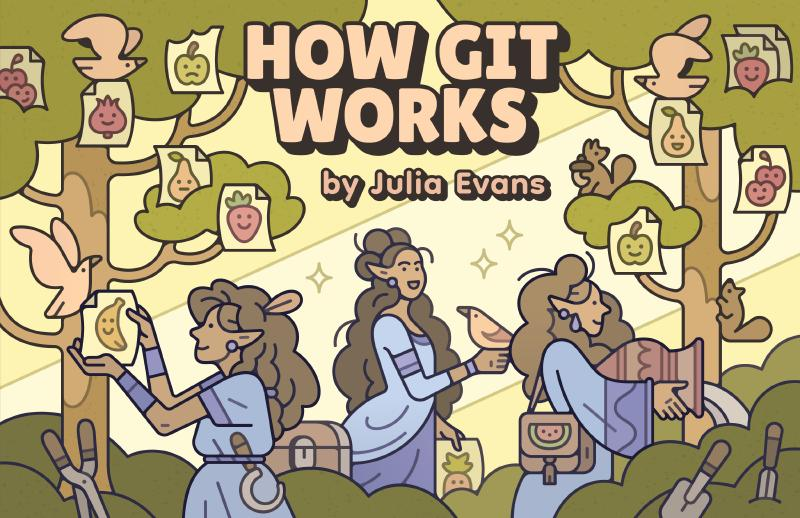
\includegraphics[height=0.5\textheight]{images/how-git-works-book-cover.jpg}
    }
\end{frame}

\begin{frame}[fragile]{Online resources}
    This is a tiny selection of the wealth of information that exists online
    about Git.
    \begin{itemize}
        \item Pro Git book: \url{https://git-scm.com/book/en/v2}
        \item Git reference documentation: \url{https://git-scm.com/docs}
        \item Cheat sheet: \url{https://git-scm.com/cheat-sheet}
    \end{itemize}
\end{frame}

\begin{frame}[fragile]{Git's built-in help}
    Git provides extensive documentation, included as part of the standard
    installation.

    Show basic usage information:
    \begin{minted}{text}
        git help
    \end{minted}

    Show detailed subcommand documentation, e.g.\ for the \code{commit}
    subcommand:
    \begin{minted}{text}
        git help commit
    \end{minted}

    or, equivalently:
    \begin{minted}{text}
        git commit --help
    \end{minted}
\end{frame}

\begin{frame}[fragile]{Git's built-in help}
    On Linux, or Windows via WSL, detailed subcommand documentation is
    provided by the appropriate man page.

    Windows via GitBash or PowerShell opens a web browser pointing to a
    local web page of the same information.

    Try it out!

    Run these commands and browse through the output:
    \begin{minted}{text}
        git help add
        git status --help
        man git commit  # only on Linux or WSL
    \end{minted}
    Your goal: get a feel for what the built-in documentation looks like.
\end{frame}

\subsection{Deleting files}

\begin{frame}[fragile]{The pav' needs to go}
    Unfortunately, the pavlova doesn't sell as well as we'd hoped.

    Also, it's the cake that takes the most work to make.

    We've discussed this with our chef and have decided to remove it from
    our selection of cakes.

    How do we do this?
\end{frame}

\begin{frame}[fragile]{The pav' needs to go}
    In Git, we delete files with the \code{git rm} command.  The \code{rm}
    part is short for \emph{remove}.

    Let's try this now and remove the pavlova recipe file.
    \begin{shellcode}
        git rm sweet/pavlova.md
    \end{shellcode}
    \begin{outputcode}
        rm 'recipes/sweet/pavlova.md'
    \end{outputcode}

    Git shows the operation it performed: the Unix-like \code{rm} command.

    This changes the repository state:
    \begin{shellcode}
        git status
    \end{shellcode}
    \begin{outputcode}
On branch main
Changes to be committed:
  (use "git restore --staged <file>..." to unstage)
        deleted:    sweet/pavlova.md
    \end{outputcode}
    Note: Git also shows us how to undo the deletion!
\end{frame}

\begin{frame}[fragile]{The pav' needs to go}
    Running \code{git rm} only changed the repository state, we have to
    commit that to make it permanent:
    \begin{shellcode}
        git commit
    \end{shellcode}
    \begin{outputcode}
[main 49d1868] Remove now unnecessary pavlova recipe
 1 file changed, 23 deletions(-)
 delete mode 100644 recipes/sweet/pavlova.md
    \end{outputcode}
    Where we also mentioned in the commit message \emph{why} this change was
    necessary.

    \begin{shellcode}
        git log -1  # show log of last commit
    \end{shellcode}
    \begin{outputcode}
commit 49d1868a9dd84bd838fa329b0c0c9f4aaab56a75 (HEAD -> main)
Author: Paul Cochrane <paul@peateasea.de>
Date:   Thu Oct 1 17:10:52 2026 +0000

    Remove now unnecessary pavlova recipe

    We found that this cake didn't sell so well and it's a lot of work to
    make, hence we're removing it from our selection of cakes.
    \end{outputcode}
\end{frame}

\begin{frame}[fragile]{Important points about \texttt{git rm}}
    Note that \code{git rm} does \emph{not} remove the files from the
    repository.  It only removes them from the working copy.  The file can
    still be accessed by checking out an earlier commit.

    \emoji{bomb} Be careful what you add to a repository!  Once committed,
    it's always available!

    \emoji{thumbs-up} This is great to retrieve old work or accidentally
    deleted files.

    \emoji{stop-sign} DO NOT add sensitive information such as passwords to
    the repository!
\end{frame}

\subsection{The three faces of a Git repository}

\begin{frame}[fragile]{The three faces of a Git repository}
    There are three aspects to a Git repository:
    \begin{itemize}
        \item the working copy
        \item the staging area
        \item the repository
    \end{itemize}

    The word ``repository'' is used in two senses here.

    One is very specific: it is the \code{.git} directory where the content
    is stored.

    The other, more loose term, encompasses the working copy, staging area
    and the \code{.git} directory repository.

    The repository is really only the \code{.git} directory and its content.
    However, we often say ``the repository'' when we mean the project
    directory.
\end{frame}

\begin{frame}[fragile]{The working copy}
    The files we see when we run \code{ls} (or \code{dir} in PowerShell) is
    referred to as the \emph{working copy}.

    This is where we make changes to project files that we later wish to
    store in the repository as a commit.  I.e.\  they're the files that
    we're ``working on'', hence the name \emph{working copy}.

    For example, from our \code{kiwi-cakes-and-coffee} project:
    \begin{outputcode}
recipes
├── savoury
│   ├── bacon-and-egg-pie.md
│   └── cheese-scones.md
└── sweet
    ├── chocolate-cake.md
    └── kiwi-cheesecake.md
    \end{outputcode}

    Note: the working copy also called the \emph{working directory} or the
    \emph{working tree}.  These are all terms for the same thing.
\end{frame}

\begin{frame}[fragile]{The staging area}
    In general, before we commit changes to the repository, we move them
    from the working copy into the \emph{staging area}.

    Adding file changes to the staging area is called \emph{staging}.
    Removing staged changes is called \emph{unstaging}.

    We've seen the word \emph{staged} in the output from \code{git status}
    after using e.g.\ \code{git add} or \code{git rm}.

    For instance, from earlier:
    \begin{minted}[fontsize=\tiny, escapeinside=||]{output}
        On branch main
        Changes not |\textbf{staged}| for commit:
          (use "git add <file>..." to update what will be committed)
          (use "git restore <file>..." to discard changes in working directory)
                modified:   chocolate-cake.md
                modified:   pavlova.md
                modified:   sour-cream-cheesecake.md

        no changes added to commit (use "git add" and/or "git commit -a")
    \end{minted}
\end{frame}

\begin{frame}[fragile]{The staging area}
    Note: due to historical reasons, the staging area is also called the
    \emph{index} or the \emph{cache}.

    E.g.\ to see a diff of the changes in the staging area, one uses:
    \begin{shellcode}
        git diff --cached
    \end{shellcode}

    The \code{git status} output can even use both terms at once:
    \begin{minted}[fontsize=\tiny, escapeinside=||]{output}
        Changes to be committed:
          (use "git rm --|\textbf{cached}| <file>..." to |\textbf{unstage}|)
                new file:   recipes/chocolate-cake.md
    \end{minted}

    Yes, this can be confusing.  \emoji{confused-face}  Sorry about that!
\end{frame}

\begin{frame}[fragile]{The repository}
    Where snapshots of project state (i.e.\ \emph{commits}) are stored.

    It's just a directory with lots of files.

    For example:
    \begin{shellcode}
        ls .git
    \end{shellcode}
    \begin{outputcode}
COMMIT_EDITMSG
HEAD
branches/
config
description
hooks/
index
info/
logs/
objects/
refs/
    \end{outputcode}

    Simple!
\end{frame}

\begin{frame}[fragile]{Three components visually related}
    tikz image...
    working copy -> staging area -> repository
\end{frame}

\begin{frame}[fragile]{But why the separation?}
    Why not just commit directly?

    Why have the staging area at all?

    It's possible to commit changes directly to the repository, and we've
    already done that:
    \begin{shellcode}
        git commit <files>
    \end{shellcode}

    However, one often wishes to select a subset of changes from the working
    copy and collect these into a commit.  This ``middle ground'' is used
    to pre-select and organise changes before committing them.

    The staging area is perfect for this use case and can be used if
    one wants to.
\end{frame}

\subsection{Recap: the three stages of a commit}

\begin{frame}[fragile]{Recap: the three stages of a commit}
    A common workflow when working with Git:
    \begin{enumerate}
        \item Edit files in the working copy.
        \item Move changes from the working copy to the staging area
            (e.g.\ \code{git add}, \code{git rm}, \code{git mv}).
        \item Save the collected changes from the staging area as a snapshot
            in the repository (\code{git commit}).
    \end{enumerate}
\end{frame}

\subsection{Commits and commit messages}

\begin{frame}[fragile]{What goes into a commit?}
    A common question: \emph{what goes into a commit?}

    The exact answer depends on experience, team dynamics and project rules.

    The best advice:

    \begin{quote}
        A commit encompasses a single, self-contained idea.
    \end{quote}

    Note that the idea can encompass:
    \begin{itemize}
        \item a single file,
        \item a bundle of many files,
        \item a part of a single file,
        \item or several separate elements of different files.
    \end{itemize}

    In general, it depends.  The course examples try to show good best
    practices.
\end{frame}

\begin{frame}[fragile]{How often should I commit?}
    How often should one commit new changes?
    \begin{itemize}
        \item as often as possible
        \item ``release early, release often''
        \item as soon as the changes belonging to a given idea are
            finished
        \item small ``atomic'' commits have smaller diffs and are easier for
            others to review
        \item don't be afraid to commit!
    \end{itemize}

    See also Seth Robertson's list of Git best practices:
    {\footnotesize \url{http://sethrobertson.github.io/GitBestPractices}}.
\end{frame}

\begin{frame}[fragile]{Writing good commit messages}
    A commit message has two parts:
    \begin{itemize}
        \item a subject line,
        \item and a body.
    \end{itemize}
    Important: these are separated by a \emph{single, blank line}.

    The \textbf{subject} is a short, concise summary of the changes
    implemented in the commit.

    The \textbf{body} explains \emph{why} the commit is important as well as
    any related context which might not be clear from the code changes
    themselves.

    See also advice from Vim guru Tim Pope:\\
    {\footnotesize \url{https://tbaggery.com/2008/04/19/a-note-about-git-commit-messages.html}}
\end{frame}

\begin{frame}[fragile]{Writing good commit messages}
    Good commit messages are an important part of communication within a
    project.

    The message should be able to clearly explain at some later time what
    happened in the change.

    When problems occur, the commit message is the first place one looks for
    information.

    They are not only messages to other people, they are also messages to
    yourself in the future.

    Advice: be nice to your future self and your colleagues and take the
    time to write well considered commit messages!
\end{frame}

\begin{frame}
\frametitle{Ignoring files}

To ignore files in Git one simply needs a \code{.gitignore} file with
entries for the files one wishes to ignore. It is possible to use
regular expressions and wildcards such as \code{*.o} in order to ignore
multiple files.

TODO: insert example of creating files to ignore and then creating a
\code{.gitignore} file.
\end{frame}

\begin{frame}[fragile]
\frametitle{Ignoring files (cont.)}

Because the \code{.gitignore} file can change (and it’s highly likely
that we’re interested in these changes) one also keeps this file under
version control. We therefore add the file to the repository and commit
it:

    \inputminted{bash}{add-gitignore.txt}
\end{frame}

\begin{frame}[fragile]
\frametitle{Showing branches (cont.)}
\code{git branch} shows available branches and which branch is
current.

    \inputminted{bash}{git-branch-output.txt}

\code{git branch -v} shows the commit hash and the commit
message of the most recent commit.

TODO need more expansive examples here with multiple branches.

    \inputminted{bash}{git-branch-v-output.txt}
\end{frame}
